\section{Aktørbeskrivelse}

I det følgende afsnit kan der læses om de aktører, der er tilknyttet systemet. \\

\begin{figure}[H]
	\centering
	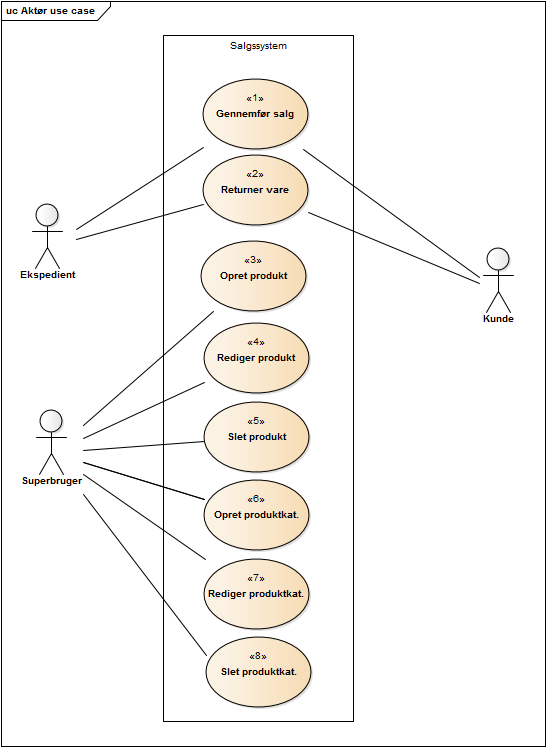
\includegraphics[width=0.6\textwidth]{Krav/Images/AktorUC}
	\caption{Use Cases med aktører}
	\label{fig:ActorUC}
\end{figure}

\begin{table}[H]
	\label{EKS}
	\begin{tabularx}{\textwidth}{|l|X|}
		\hline
		\textbf{Navn} & Ekspedient \\
		\hline
		\textbf{Type} & Primær \\
		\hline
		\textbf{Beskrivelse} & Ekspedient er en primær bruger af systemet, som benytter systemet til at sælge og returnere vare. \\
		\hline
	\end{tabularx}
	\captionsetup{justification=raggedright,singlelinecheck=false}
	\caption{Aktørbeskrivelse af Ekspedient}
	\label{tab:AktEks}
\end{table}


\begin{table}[H]
	\begin{tabularx}{\textwidth}{|l|X|}
		\hline
		\textbf{Navn} & Superbruger \\
		\hline
		\textbf{Type} & Primær \\
		\hline
		\textbf{Beskrivelse} & Superbruger er en primær bruger af systemet, som benytter systemet til at oprette, nedlægge og redigere i systemets varekatalog. \\
		\hline
	\end{tabularx}
	\captionsetup{justification=raggedright,singlelinecheck=false}
	\caption{Aktørbeskrivelse af Superbruger}
	\label{tab:AktSuu}
\end{table}

\begin{table}[H]
	\label{KD}
	\begin{tabularx}{\textwidth}{|l|X|}
		\hline
		\textbf{Navn} & Kunde \\
		\hline
		\textbf{Type} & Sekundær \\
		\hline
		\textbf{Beskrivelse} & Kunden er en sekundær bruger af systemet, og ønsker at købe/returnere en eller flere varer igennem Ekspedienten. Ekspedienten er beskrevet i tabel \ref{EKS}.   \\
		\hline
	\end{tabularx}
	\captionsetup{justification=raggedright,singlelinecheck=false}
	\caption{Aktørbeskrivelse af Kunde}
	\label{tab:AktKu}
\end{table}
